% !TEX root = ../thesis.tex

\chapter{Summary and Prospect}

\section{Summary}

This undergraduate thesis investigated LCh molecule model, a typical kind of liquid crystal with helix interactions. In principle, they are supposed to behave isotropically under under high temperature or very low density, which is the isotropic phase and anisotropically under high density or low temperature where molecules are oriented preferably in a certain direction. And further if they have chiral mutual interactions between each other, they tend to lean on each other with a preferable non zero angle, behaving periodically in the space, which is the cholesteric phase. These phenomena are observed in both experiments and simulations\cite{Liang2017SM}. So a theoretical method is developed in this thesis to give a prediction of the thermodynamic properties of FCh model. The theory is based on Onsager's original theory\cite{Onsager1949NYAS} of phase transition of liquid crystals, and makes use of DFT method to give a depiction of the thermodynamic properties of the phase transition of FCh. In addition, a modular program is developed from scratch for the phase diagram computation of a wide range of liquid crystal molecules including FCh.

\section{Prospect on Computation of RDF}
As is stated in the previous chapter, the lack of accurate RDF accounts that the transition density of theory is slightly larger that that of the theory. We then tried to solve the radial distribution function (RDF) for FCh model, using the Percus-Yevick equation, we write the overall ideas and difficulties. Hope those who are interested in the study of RDF focus on the essential problem raised here.

The Ornstein-Zernike equation is proposed to solve the radial distribution function (RDF), let $h(r)=g(r)-1$ be the total correlation function, then it can be split into two parts according to Ornstein and Zernike\cite{Ornstein1914OZeqn},
\begin{equation}
	h(|r_1-r_2|)=c(|r_1-r_2|)+n\int\on{d}r_3c(|r_1-r_3|)h(|r_3-r_3|)
\end{equation}
in which $c(r)$ is the direct correlation. Then the Percus-Yevick approximation gives $c(r)=f(r)y(r)$, $f(r)=e^{-\beta u(r)}-1$ is the Mayer's function, $y(r)=e^{\beta u(r)}g(r)$ is the background correlation function. Then the Percus-Yevick equation is given by
\begin{equation}\label{Eqn:OrdPY}
	y(|r_1-r_2|)=1+n\int\on{d}r_3f(|r_1-r_3|)y(|r_1-r_3|)h(|r_2-r_3|).
\end{equation}

The equation has an analytic solution for hard spheres according to Wertheim\cite{Wertheim1963HS}. Lago et al. also have great work\cite{Lago2003SQSC} on the approximate solution of Percus-Yevick equation of square well spherocylinders. To be more precise, the OZ and PY equation for a rod-like molecule should be modified as follows:
\begin{equation}
	\begin{split}
		h(r_1,u_1;r_2,u_2)=c(r_1,u_1;r_2,u_2)+n\int\on{d}r_3\frac{\on{d}u_3}{4\pi} h(r_1,u_1;r_3,u_3)c(r_2,u_2;r_3,u_3)\\
		y(r_1,u_1;r_2,u_2)=1+n\int\on{d}r_3\frac{\on{d}u_3}{4\pi}f(r_1,u_1;r_3,u_3)y(r_1,u_1;r_3,u_3)h(r_2,u_2;r_3,u_3).
	\end{split}
\end{equation}
And the Percus-Yevick approximation is as same as the preceding one. To decouple the distance parameter and orientation parameter, Lago et al. used an interpolation method to split the background correlation in four main parts, i.e.
\begin{equation}\label{Eqn:splitY}
	\begin{split}
	y\left(r, \alpha, \beta, \theta\right)=& y_{HT}\left(r\right)+\left[y_{P}\left(r\right)-y_{HT}\left(r_{12}\right)\right] \sin \theta \\
	&+\left[y_{C}\left(r\right)-y_{P}\left(r\right)\right] \sin \alpha \\
	&+\left[y_{T}\left(r\right)-y_{P}\left(r\right)\right] \sin \beta.
	\end{split}
\end{equation}
In the equations, $\alpha,\beta,\theta$ are defined in Fig. \ref{fig:lago}. And $HT$ means head-to-tail configuration, $P$ means parallel, $C$ means cross, and $T$ means T-shape. And they can be solved respectively (this is not clear in the original paper), we logically infer to solve them individually, it suffices to solve four integral equation simultaneously (using $(i,j)$ to represent $(r_i,u_i,\phi_i;r_j,u_j,\phi_j)$):
\begin{equation}
	\begin{split}
		y_{HT}(12)&=1+n\int\on{d}r_3\frac{\on{d}u_3}{4\pi}f(13)y(13)h(23), \text{with 1 and 2 are chosen to be head to tail} \\
		y_{P}(12)&=1+n\int\on{d}r_3\frac{\on{d}u_3}{4\pi}f(13)y(13)h(23), \text{with 1 and 2 are chosen to be parallel} \\
		y_{C}(12)&=1+n\int\on{d}r_3\frac{\on{d}u_3}{4\pi}f(13)y(13)h(23), \text{with 1 and 2 are chosen to be cross} \\
		y_{T}(12)&=1+n\int\on{d}r_3\frac{\on{d}u_3}{4\pi}f(13)y(13)h(23), \text{with 1 and 2 are chosen to be T-shape} 
	\end{split}
\end{equation}
Together with Eqn. \ref{Eqn:splitY}, the four integral equation can be solved by iteration method in principal, but very hard and time-consuming in practice.
\begin{figure}[H]
 	\centering
 	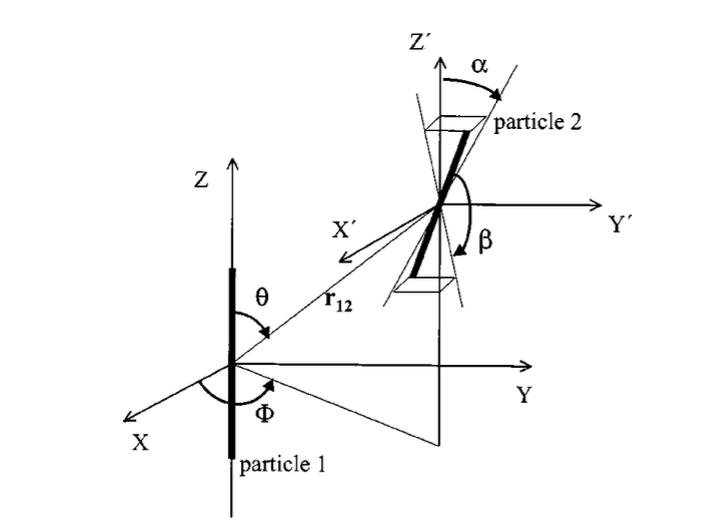
\includegraphics[width=\linewidth]{lago03.png} \\
	\caption[Schematic of coordinates]{Schematic figure of relative coordinates\cite{Liang2019PRE}}
	\label{fig:lago}
\end{figure}

If we tried to apply to FCh molecule,  since it has an additional parameter, the internal azimuthal angle $\phi$ involved in the integral, namely $\dfrac{\on{d}\phi}{2\pi}$. The solution of the four integral equations becomes much more impractical.


